% ──────────────────────────────────────────────────────────────
\subsection{Ecosistema Digital Electoral}
% ──────────────────────────────────────────────────────────────
 
El ecosistema digital electoral es el conjunto de plataformas, actores y flujos de información que operan en el entorno digital durante un proceso electoral, y a través del cual los ciudadanos expresan opiniones, debaten propuestas, comparten noticias y construyen o destruyen la imagen pública de los candidatos \parencite{mc_chadwick2013hybrid}. A diferencia de los medios tradicionales —prensa escrita, radio y televisión—, este ecosistema se caracteriza por la descentralización de la producción de contenido, la velocidad casi instantánea de difusión y la posibilidad de interacción directa entre ciudadanos y actores políticos.
 
El ecosistema digital electoral está compuesto por tres tipos de actores. Los \textbf{actores institucionales} incluyen partidos políticos, candidatos y organismos electorales que utilizan las plataformas digitales de manera estratégica para comunicar sus propuestas y movilizar votantes. Los \textbf{actores mediáticos digitales} son los medios de comunicación nativos digitales, blogs especializados y portales de noticias que cubren la campaña en tiempo real. Finalmente, los \textbf{ciudadanos} son quienes generan el mayor volumen de contenido a través de sus publicaciones, comentarios y reacciones en redes sociales, constituyendo la fuente primaria de datos para los sistemas de inteligencia electoral \parencite{mc_ceron2017social}.
 
La comprensión de este ecosistema es fundamental para la presente investigación, ya que los datos recolectados para el análisis de percepción pública nacional provienen de las interacciones que tienen lugar en él.
 
% ──────────────────────────────────────────────────────────────
\subsection{Percepción Pública}
% ──────────────────────────────────────────────────────────────
 
La percepción pública es el proceso cognitivo y evaluativo mediante el cual la ciudadanía forma juicios colectivos sobre personas, instituciones, eventos o políticas públicas, a partir de la información disponible en su entorno \parencite{mc_lippmann1922public}. En el contexto electoral, la percepción pública se manifiesta en las actitudes que los ciudadanos expresan hacia los candidatos, los partidos políticos, las propuestas programáticas y los resultados de gestión de los gobiernos.
 
Tradicionalmente, la percepción pública se medía mediante encuestas de opinión y grupos focales. Sin embargo, el auge de las redes sociales ha generado un flujo continuo y masivo de expresiones ciudadanas que constituyen un indicador alternativo —y complementario— de la percepción pública, con ventajas significativas: es ininterrumpido, de bajo costo, de alta escala y capaz de capturar cambios en tiempo real asociados a eventos específicos de la campaña \parencite{mc_ceron2017social}.
 
En el marco de esta investigación, la percepción pública nacional se operacionaliza como el conjunto de sentimientos, emociones y evaluaciones que los ciudadanos peruanos expresan en ecosistemas digitales en relación con el proceso electoral en curso, medidos a través de las técnicas de minería de sentimientos descritas en el presente trabajo.
 
% ──────────────────────────────────────────────────────────────
\subsection{Minería de Sentimientos}
% ──────────────────────────────────────────────────────────────
 
La minería de sentimientos, también conocida como análisis de sentimientos u opinión mining, es la disciplina del Procesamiento del Lenguaje Natural orientada a identificar, extraer y cuantificar automáticamente las actitudes subjetivas expresadas en textos digitales —sean estas positivas, negativas o neutras— hacia personas, entidades, productos, eventos o temas de interés \parencite{mc_liu2012sentiment}. Va más allá de la simple clasificación de polaridad al buscar identificar también la intensidad del sentimiento, la emoción subyacente y las entidades específicas hacia las que se dirigen dichas actitudes.
 
En el contexto de la inteligencia electoral, la minería de sentimientos permite responder preguntas como: ¿Qué proporción de la conversación digital expresa apoyo o rechazo hacia un candidato? ¿Cómo varía el sentimiento ciudadano antes y después de un debate presidencial? ¿Qué emociones predominan en la discusión sobre una propuesta de política pública? Las respuestas a estas preguntas ofrecen información valiosa y complementaria a las encuestas convencionales para la comprensión de la dinámica electoral \parencite{mc_ceron2017social}.
 
Formalmente, dado un conjunto de documentos $D = \{d_1, d_2, \ldots, d_n\}$, la minería de sentimientos busca asignar a cada documento $d_i$ una función de sentimiento $S(d_i, e_j) \in \{positivo, negativo, neutro\}$, donde $e_j$ representa una entidad o aspecto de interés (por ejemplo, un candidato político), como se representa en la Figura \ref{fig:sentiment_mining_process}.
 
\begin{figure}[!ht]
    \begin{center}
        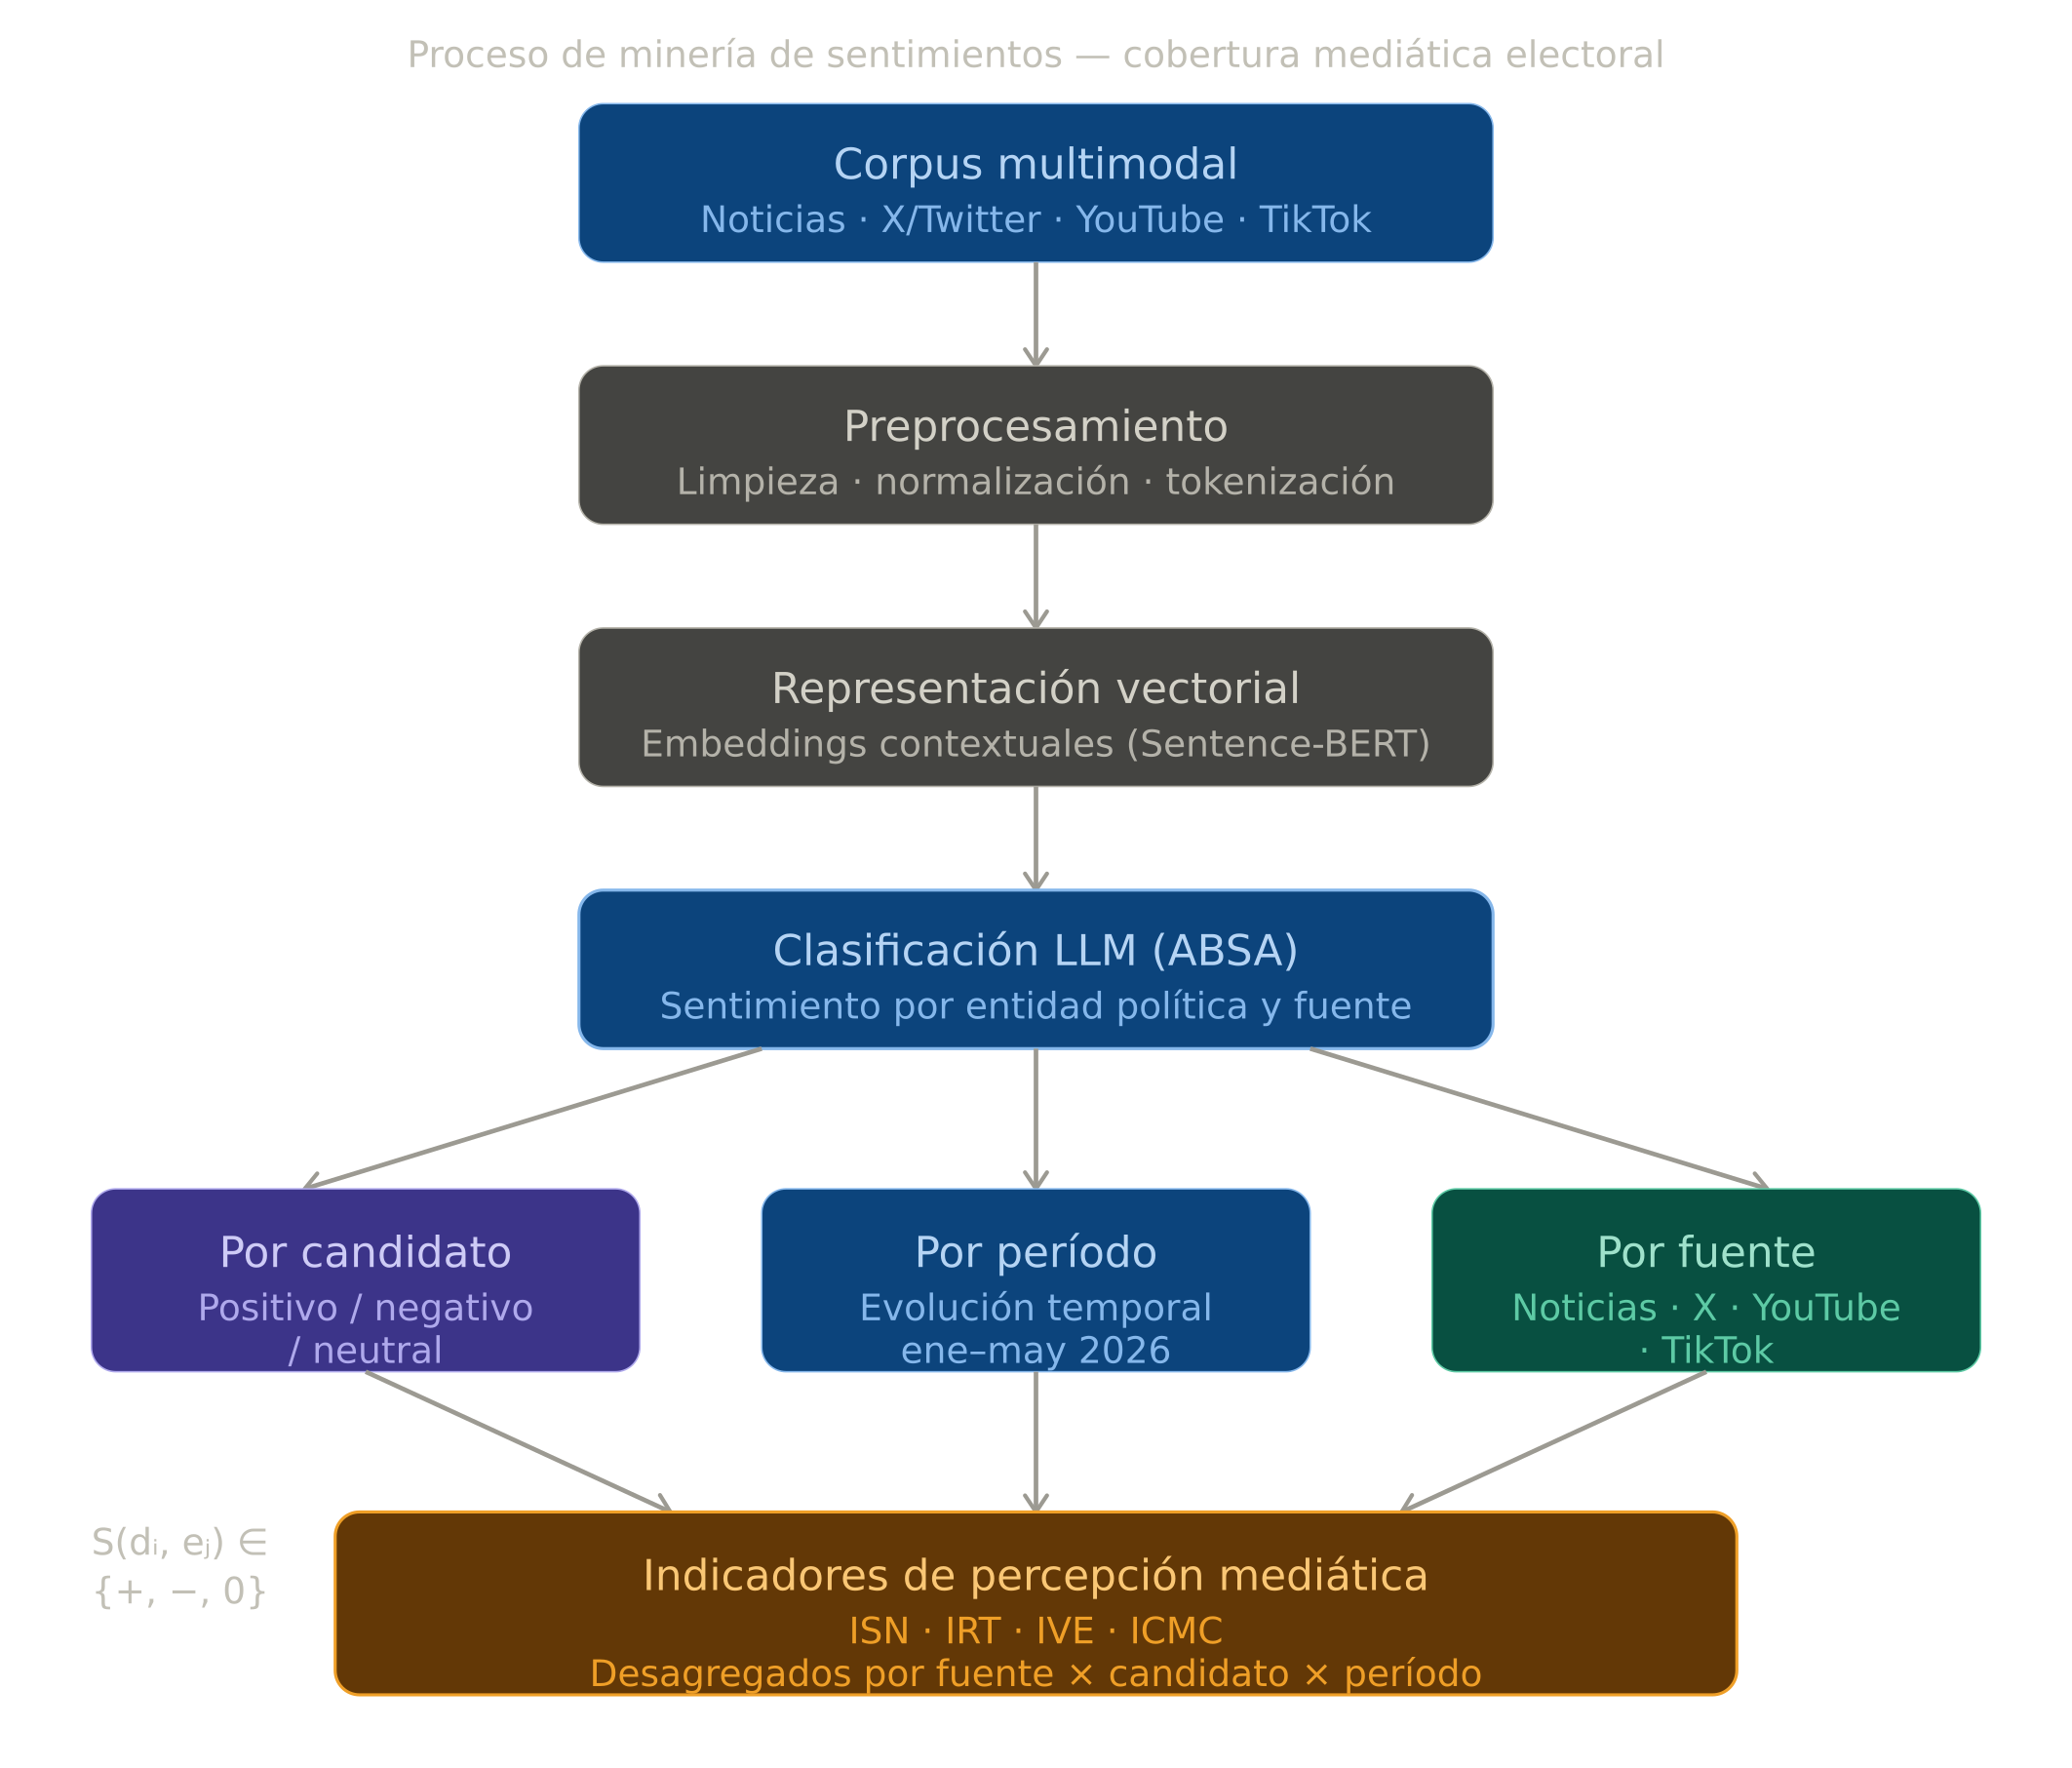
\includegraphics[width=0.85\textwidth]{2/figures/sentiment_mining_process.jpg}
        \caption[Proceso general de la minería de sentimientos aplicada al análisis electoral]{Proceso general de la minería de sentimientos en el contexto electoral: desde la recolección de publicaciones hasta la generación de indicadores de percepción pública por candidato y tema.\\
            Fuente: Elaboración propia basada en \cite{mc_liu2012sentiment}.}
        \label{fig:sentiment_mining_process}
    \end{center}
\end{figure}
 
% ──────────────────────────────────────────────────────────────
\subsection{Tema Relevante}
% ──────────────────────────────────────────────────────────────
 
En el contexto de la presente investigación, un \textbf{tema relevante} (\textit{relevant topic}) se define como un conjunto coherente de términos, conceptos y narrativas que emergen de manera recurrente en la conversación digital sobre el proceso electoral, y que refleja una preocupación, debate o acontecimiento de interés colectivo para la ciudadanía \parencite{mc_blei2012lda}. La relevancia de un tema se determina por su frecuencia relativa en el corpus de publicaciones analizadas, su persistencia en el tiempo y su capacidad de articular distintas perspectivas ciudadanas.
 
Los temas relevantes en un ecosistema digital electoral pueden agruparse en varias categorías: temas programáticos (economía, salud, educación, seguridad), temas de imagen (honestidad, liderazgo, experiencia de los candidatos), temas contingentes (escándalos, revelaciones, hechos inesperados de la campaña) y temas sistémicos (confianza en las instituciones democráticas, participación ciudadana). La capacidad de identificar y monitorear estos temas de manera automática y en tiempo real es uno de los objetivos centrales de un sistema de inteligencia electoral basado en LLMs.
 
% ──────────────────────────────────────────────────────────────
\subsection{Detección Dinámica de Temas}
% ──────────────────────────────────────────────────────────────
 
La detección dinámica de temas es la capacidad de un sistema computacional para identificar automáticamente los temas latentes presentes en un corpus de textos y rastrear su evolución a lo largo del tiempo, sin requerir etiquetado manual previo ni un conjunto predefinido de categorías temáticas \parencite{mc_grootendorst2022bertopic}. El adjetivo «dinámica» hace referencia a que el sistema es capaz de detectar no solo los temas que ya existían al inicio del período de análisis, sino también los que emergen durante el proceso como respuesta a nuevos eventos, los que se intensifican y los que decaen.
 
En el contexto electoral, la detección dinámica de temas responde a preguntas como: ¿Qué nuevos asuntos han irrumpido en la conversación digital esta semana? ¿Cuáles han perdido relevancia? ¿Existe una correlación entre la aparición de un tema y un evento específico de la campaña? Este tipo de análisis es imposible de realizar manualmente a la escala de datos generados por las redes sociales durante un proceso electoral, de ahí la necesidad de automatizarlo mediante LLMs y modelos de topic modeling como BERTopic \parencite{mc_grootendorst2022bertopic}.
 
La Figura \ref{fig:dynamic_detection_concept} ilustra el concepto de detección dinámica de temas en el contexto electoral, mostrando cómo distintos temas emergen, se intensifican y decaen a lo largo del tiempo en respuesta a los hitos de la campaña.
 
\begin{figure}[!ht]
    \begin{center}
        \includegraphics[width=0.88\textwidth]{2/figures/dynamic_detection_concept.jpg}
        \caption[Concepto de detección dinámica de temas en un proceso electoral]{Representación conceptual de la detección dinámica de temas en un proceso electoral: los temas emergen y decaen en función de los hitos de campaña (debates, anuncios, escándalos), siendo identificados automáticamente por el sistema.\\
            Fuente: Elaboración propia.}
        \label{fig:dynamic_detection_concept}
    \end{center}
\end{figure}
 
% ──────────────────────────────────────────────────────────────
\subsection{Corpus}
% ──────────────────────────────────────────────────────────────
 
En lingüística computacional y NLP, un \textbf{corpus} (plural: \textit{corpora}) es una colección estructurada y representativa de textos en formato digital, recopilados con un propósito analítico específico y que sirven como base de datos para el entrenamiento, ajuste fino o evaluación de modelos de procesamiento del lenguaje \parencite{mc_manning1999foundations}. La calidad, representatividad y tamaño del corpus son factores determinantes en la calidad de los análisis de sentimientos y detección de temas que se puedan derivar de él.
 
Para la presente investigación, el corpus está constituido por publicaciones extraídas de plataformas de redes sociales —principalmente X (antes Twitter)— relacionadas con el proceso electoral peruano, recolectadas mediante palabras clave, hashtags y cuentas de usuarios relevantes. Las características de este corpus —su tamaño, composición temporal, distribución de temas y balance entre clases de sentimiento— son descritas en detalle en el capítulo metodológico.
 
% ──────────────────────────────────────────────────────────────
\subsection{Token y Tokenización}
% ──────────────────────────────────────────────────────────────
 
Un \textbf{token} es la unidad mínima de procesamiento en la que se divide un texto para ser procesado por un modelo de NLP o un LLM. Dependiendo del tokenizador utilizado, un token puede corresponder a una palabra completa, a un subconjunto de caracteres de una palabra (\textit{subword}), a un signo de puntuación o incluso a un espacio en blanco \parencite{mc_devlin2018bert}. Los LLMs modernos utilizan tokenizadores de subpalabras como BPE (\textit{Byte Pair Encoding}) o WordPiece, que permiten manejar vocabularios abiertos y palabras fuera del vocabulario de entrenamiento.
 
La \textbf{tokenización} es el proceso de segmentar un texto de entrada en tokens antes de su procesamiento por el modelo, como se ilustra en la Figura \ref{fig:tokenization_example}. Este proceso es un paso previo indispensable en cualquier pipeline de NLP y tiene implicaciones directas en el rendimiento del modelo: textos en español político, con sus variantes léxicas regionales y uso de jerga electoral, presentan desafíos particulares de tokenización que deben ser considerados en el diseño del sistema.
 
\begin{figure}[!ht]
    \begin{center}
        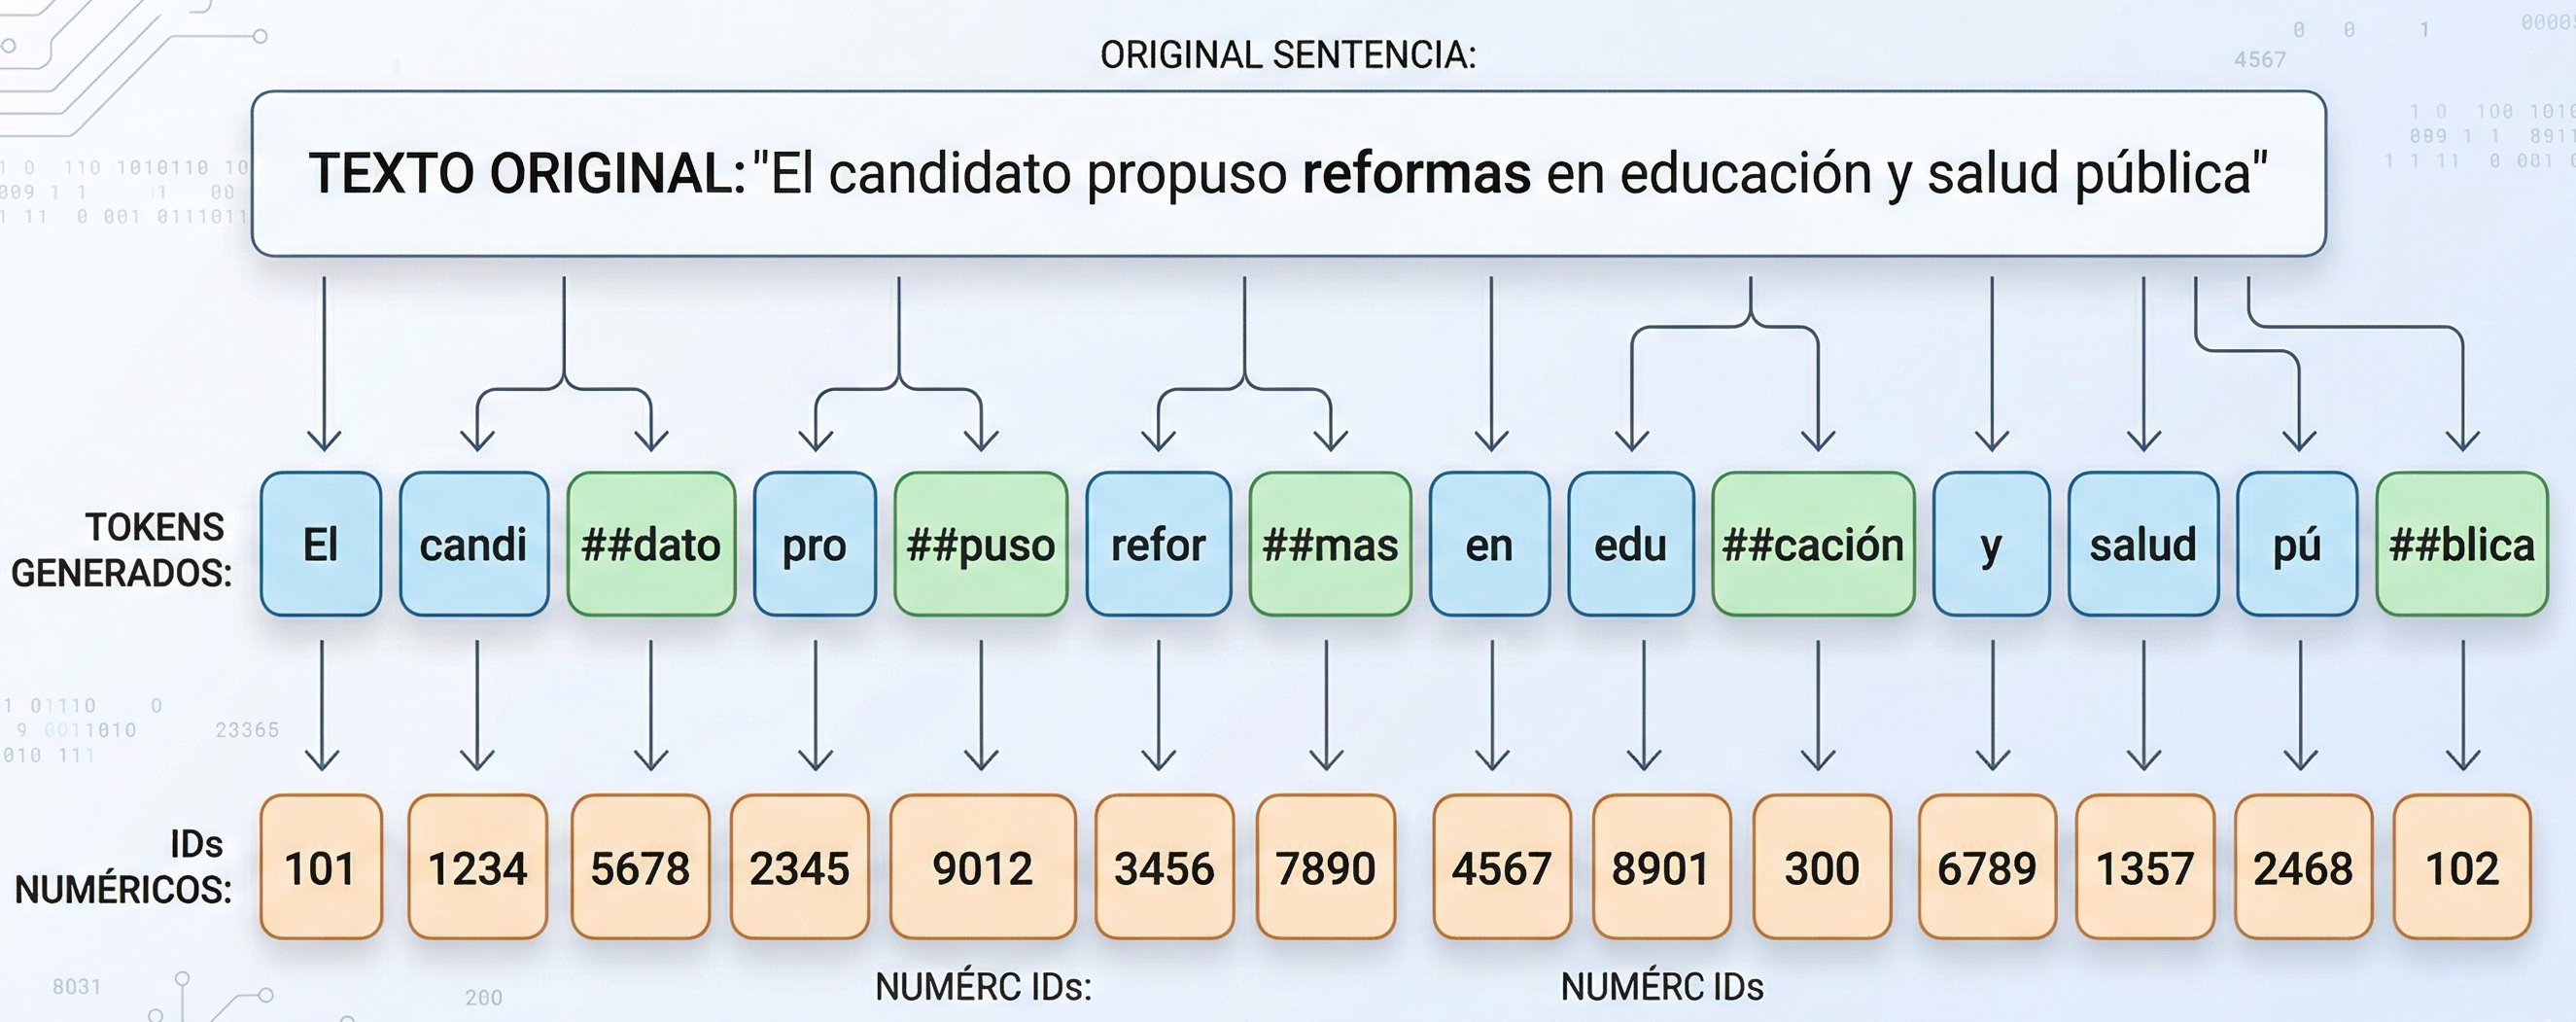
\includegraphics[width=0.82\textwidth]{2/figures/tokenization_example.jpg}
        \caption[Ejemplo de tokenización de un texto político con tokenizadores de subpalabras]{Ejemplo de tokenización BPE aplicada a un texto político en español: la oración es dividida en tokens de subpalabras que el LLM puede procesar como vectores numéricos.\\
            Fuente: Elaboración propia basada en \cite{mc_devlin2018bert}.}
        \label{fig:tokenization_example}
    \end{center}
\end{figure}
 
% ──────────────────────────────────────────────────────────────
\subsection{Embedding o Incrustación Semántica}
% ──────────────────────────────────────────────────────────────
 
Un \textbf{embedding} (o incrustación semántica) es una representación vectorial densa de un token, palabra, oración o documento en un espacio de alta dimensión, donde la proximidad geométrica entre dos vectores refleja la similitud semántica entre los elementos que representan \parencite{mc_mikolov2013word2vec}. A diferencia de las representaciones dispersas como la Bolsa de Palabras o la codificación en caliente, los embeddings capturan relaciones semánticas y sintácticas complejas en un espacio de dimensión reducida.
 
En el contexto de la presente investigación, los embeddings cumplen dos roles fundamentales. Por un lado, los \textbf{embeddings de palabras} generados por modelos como Word2Vec o GloVe permiten calcular la similitud semántica entre términos políticos y construir representaciones del vocabulario electoral. Por otro lado, los \textbf{embeddings de oraciones} generados por modelos como Sentence-BERT \parencite{mc_reimers2019sbert} constituyen la entrada al pipeline de BERTopic para la detección dinámica de temas, ya que capturan el significado global de cada publicación en un único vector denso, como se representa en la Figura \ref{fig:embedding_space}.
 
\begin{figure}[!ht]
    \begin{center}
        \includegraphics[width=0.80\textwidth]{2/figures/embedding_space.jpg}
        \caption[Espacio vectorial de embeddings de oraciones sobre discurso político electoral]{Representación del espacio vectorial de embeddings de oraciones políticas: publicaciones semánticamente similares se agrupan en regiones próximas del espacio, facilitando la posterior detección de temas mediante clustering.\\
            Fuente: Elaboración propia basada en \cite{mc_reimers2019sbert}.}
        \label{fig:embedding_space}
    \end{center}
\end{figure}
 
% ──────────────────────────────────────────────────────────────
\subsection{Prompt}
% ──────────────────────────────────────────────────────────────
 
Un \textbf{prompt} es la instrucción textual o consulta que se proporciona como entrada a un LLM para orientar y condicionar la respuesta que este genera \parencite{mc_white2023prompt}. El diseño del prompt es el mecanismo principal a través del cual el usuario comunica al modelo la tarea que debe realizar, el contexto en el que debe operar, el formato de la respuesta esperada y las restricciones que debe respetar, todo ello sin modificar los parámetros internos del modelo.
 
En el contexto de la inteligencia electoral, los prompts se utilizan para instrucciones como: «Clasifica el sentimiento de la siguiente publicación hacia el candidato X como positivo, negativo o neutro y explica brevemente tu razonamiento», o «Identifica el tema principal de las siguientes publicaciones y etiquétalo con una frase descriptiva de no más de cinco palabras». La calidad del prompt determina directamente la calidad de los resultados del sistema, razón por la cual la ingeniería de prompts es una componente técnica central de la presente investigación.
 
Los elementos clave de un prompt bien diseñado para análisis electoral incluyen: (1) la definición del \textbf{rol} del modelo («Eres un analista político experto en discurso electoral latinoamericano»), (2) el \textbf{contexto} de la tarea (el proceso electoral analizado, el idioma, las entidades relevantes), (3) la \textbf{instrucción} específica (qué debe hacer el modelo con el texto de entrada), (4) el \textbf{formato} de la respuesta esperada (JSON estructurado, categoría única, texto libre), y (5) los \textbf{ejemplos} en modalidad few-shot cuando sea necesario, como se ilustra en la Figura \ref{fig:prompt_structure}.
 
\begin{figure}[!ht]
    \begin{center}
        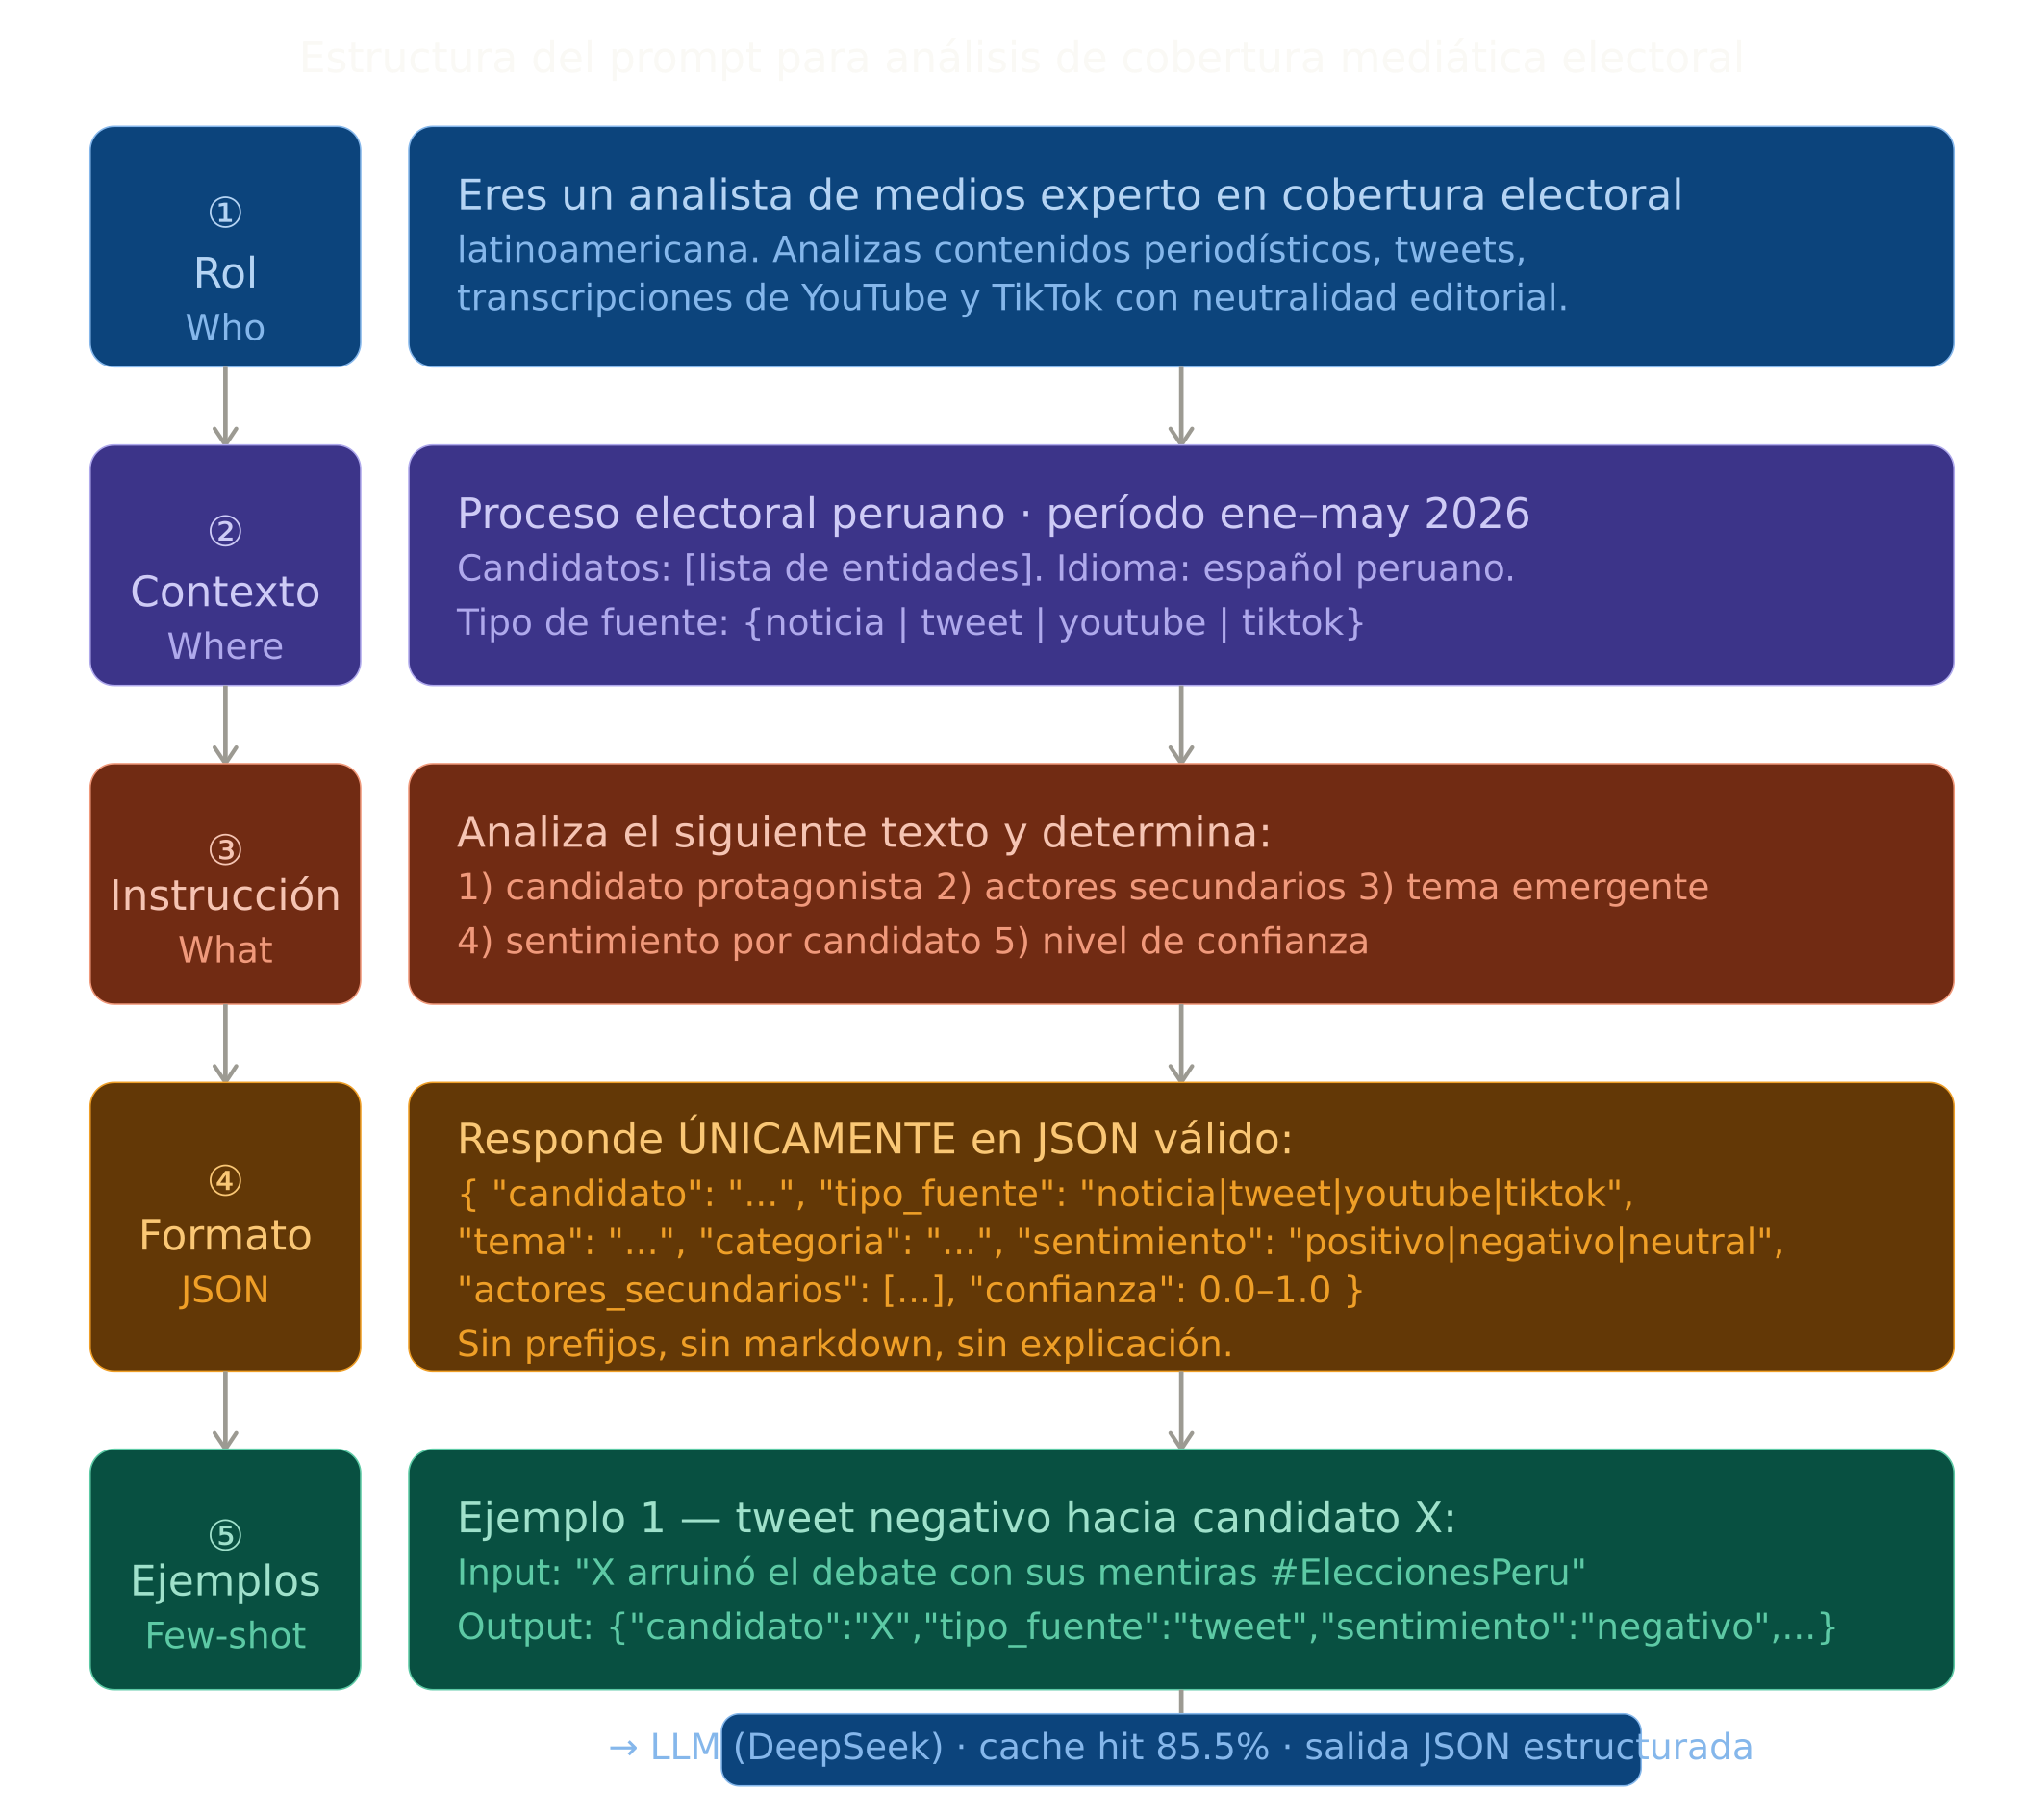
\includegraphics[width=0.85\textwidth]{2/figures/prompt_structure.jpg}
        \caption[Estructura de un prompt optimizado para análisis de sentimientos electorales]{Estructura de un prompt bien diseñado para análisis de sentimientos electorales, mostrando sus cinco componentes: rol, contexto, instrucción, formato y ejemplos few-shot.\\
            Fuente: Elaboración propia basada en \cite{mc_white2023prompt}.}
        \label{fig:prompt_structure}
    \end{center}
\end{figure}
 
% ──────────────────────────────────────────────────────────────
\subsection{Polaridad}
% ──────────────────────────────────────────────────────────────
 
La \textbf{polaridad} es la dimensión evaluativa fundamental del análisis de sentimientos, que indica la orientación afectiva de un texto hacia una entidad o aspecto determinado: positiva, negativa o neutral \parencite{mc_liu2012sentiment}. En el contexto electoral, la polaridad mide si una publicación expresa apoyo, rechazo o una posición indefinida respecto a un candidato, partido político, propuesta o evento de la campaña.
 
Más allá de la clasificación ternaria básica (positivo / negativo / neutral), existen modelos de polaridad más granulares que incluyen escalas de intensidad —muy positivo, positivo, neutral, negativo, muy negativo— o que descomponen la polaridad en sus dimensiones emocionales constituyentes (alegría, enojo, miedo, sorpresa, tristeza, asco) siguiendo modelos como el de Plutchik \parencite{mc_plutchik1980emotion}. Los LLMs modernos son capaces de operar en este nivel de granularidad emocional, lo que constituye una ventaja significativa respecto a los clasificadores binarios clásicos.
 
En el presente trabajo, la polaridad se mide a nivel de aspecto (\textit{Aspect-Based Sentiment Analysis}), es decir, desagregada por entidad política: una misma publicación puede expresar polaridad positiva hacia una propuesta económica y negativa hacia la gestión en seguridad de un mismo candidato, capturando así la complejidad real del discurso político ciudadano.
 
% ──────────────────────────────────────────────────────────────
\subsection{Desinformación Electoral}
% ──────────────────────────────────────────────────────────────
 
La \textbf{desinformación electoral} es la producción y difusión deliberada de contenido falso, engañoso o manipulado con el propósito de distorsionar la percepción pública sobre candidatos, procesos electorales o resultados, con el fin de influir en el comportamiento de los votantes o deslegitimar las instituciones democráticas \parencite{mc_wardle2017information}. Se distingue de la \textbf{desinformación involuntaria} (\textit{misinformation}), que corresponde a la difusión de contenido falso sin intención de engañar.
 
En el ecosistema digital, la desinformación electoral puede adoptar múltiples formas: noticias falsas fabricadas (\textit{fake news}), imágenes o videos manipulados (\textit{deepfakes}), cuentas automatizadas (\textit{bots}) que amplifican artificialmente narrativas, o titulares descontextualizados que distorsionan hechos reales \parencite{pr_chen2024combating_misinformation}. La irrupción de los LLMs ha agravado este problema al facilitar la generación masiva de texto de apariencia creíble, aunque también ha abierto nuevas posibilidades para su detección automatizada mediante los mismos modelos.
 
En el sistema de inteligencia electoral propuesto en esta investigación, la detección de desinformación opera como un módulo complementario al análisis de sentimientos y la detección de temas, con el objetivo de garantizar que los indicadores de percepción pública no sean distorsionados por contenido falso amplificado artificialmente.
 
% ──────────────────────────────────────────────────────────────
\subsection{Polarización Política Digital}
% ──────────────────────────────────────────────────────────────
 
La \textbf{polarización política digital} es el fenómeno por el cual las conversaciones en ecosistemas digitales tienden a organizarse en dos o más grupos ideológicamente distantes, con escasa interacción entre ellos y con una progresiva intensificación del discurso afectivo negativo hacia el grupo contrario \parencite{mc_iyengar2019origins}. Este fenómeno, que en la literatura anglosajona se denomina también \textit{affective polarization} (polarización afectiva), es amplificado por los algoritmos de recomendación de las plataformas digitales, que tienden a reforzar las preferencias existentes de los usuarios en lugar de exponerlos a perspectivas diversas.
 
En el contexto de la inteligencia electoral, la medición de la polarización política digital es un indicador relevante de la salud del ecosistema de debate público: niveles extremos de polarización se asocian con mayor susceptibilidad a la desinformación, menor disposición al diálogo ciudadano y mayor volatilidad del comportamiento electoral \parencite{mc_iyengar2019origins}. Los LLMs permiten cuantificar la polarización a través del análisis de la distribución y la intensidad del sentimiento negativo entre grupos de usuarios y del monitoreo de las narrativas que cada grupo construye sobre el otro.
 
% ──────────────────────────────────────────────────────────────
\subsection{Monitoreo en Tiempo Real}
% ──────────────────────────────────────────────────────────────
 
El \textbf{monitoreo en tiempo real} (\textit{real-time monitoring}) es la capacidad de un sistema computacional para ingerir, procesar y analizar flujos continuos de datos digitales con una latencia mínima, generando resultados actualizados de manera casi instantánea \parencite{mc_garcia2025real_time}. En el contexto de la inteligencia electoral, esto significa que el sistema es capaz de detectar un cambio brusco en el sentimiento ciudadano o la emergencia de un nuevo tema en el ecosistema digital en cuestión de minutos desde que el evento desencadenante ocurre, permitiendo a los analistas políticos y periodistas actuar sobre información actualizada.
 
El monitoreo en tiempo real requiere una arquitectura de software específica que incluye: (1) un módulo de ingesta de datos en streaming (por ejemplo, mediante la API de X/Twitter Filtered Stream), (2) un módulo de preprocesamiento que limpia y normaliza el texto a medida que llega, (3) un módulo de inferencia con el LLM que clasifica sentimientos y detecta temas de manera paralela, y (4) un módulo de visualización que actualiza los dashboards en tiempo real con los nuevos resultados, como se esquematiza en la Figura \ref{fig:realtime_architecture}.
 
\begin{figure}[!ht]
    \begin{center}
        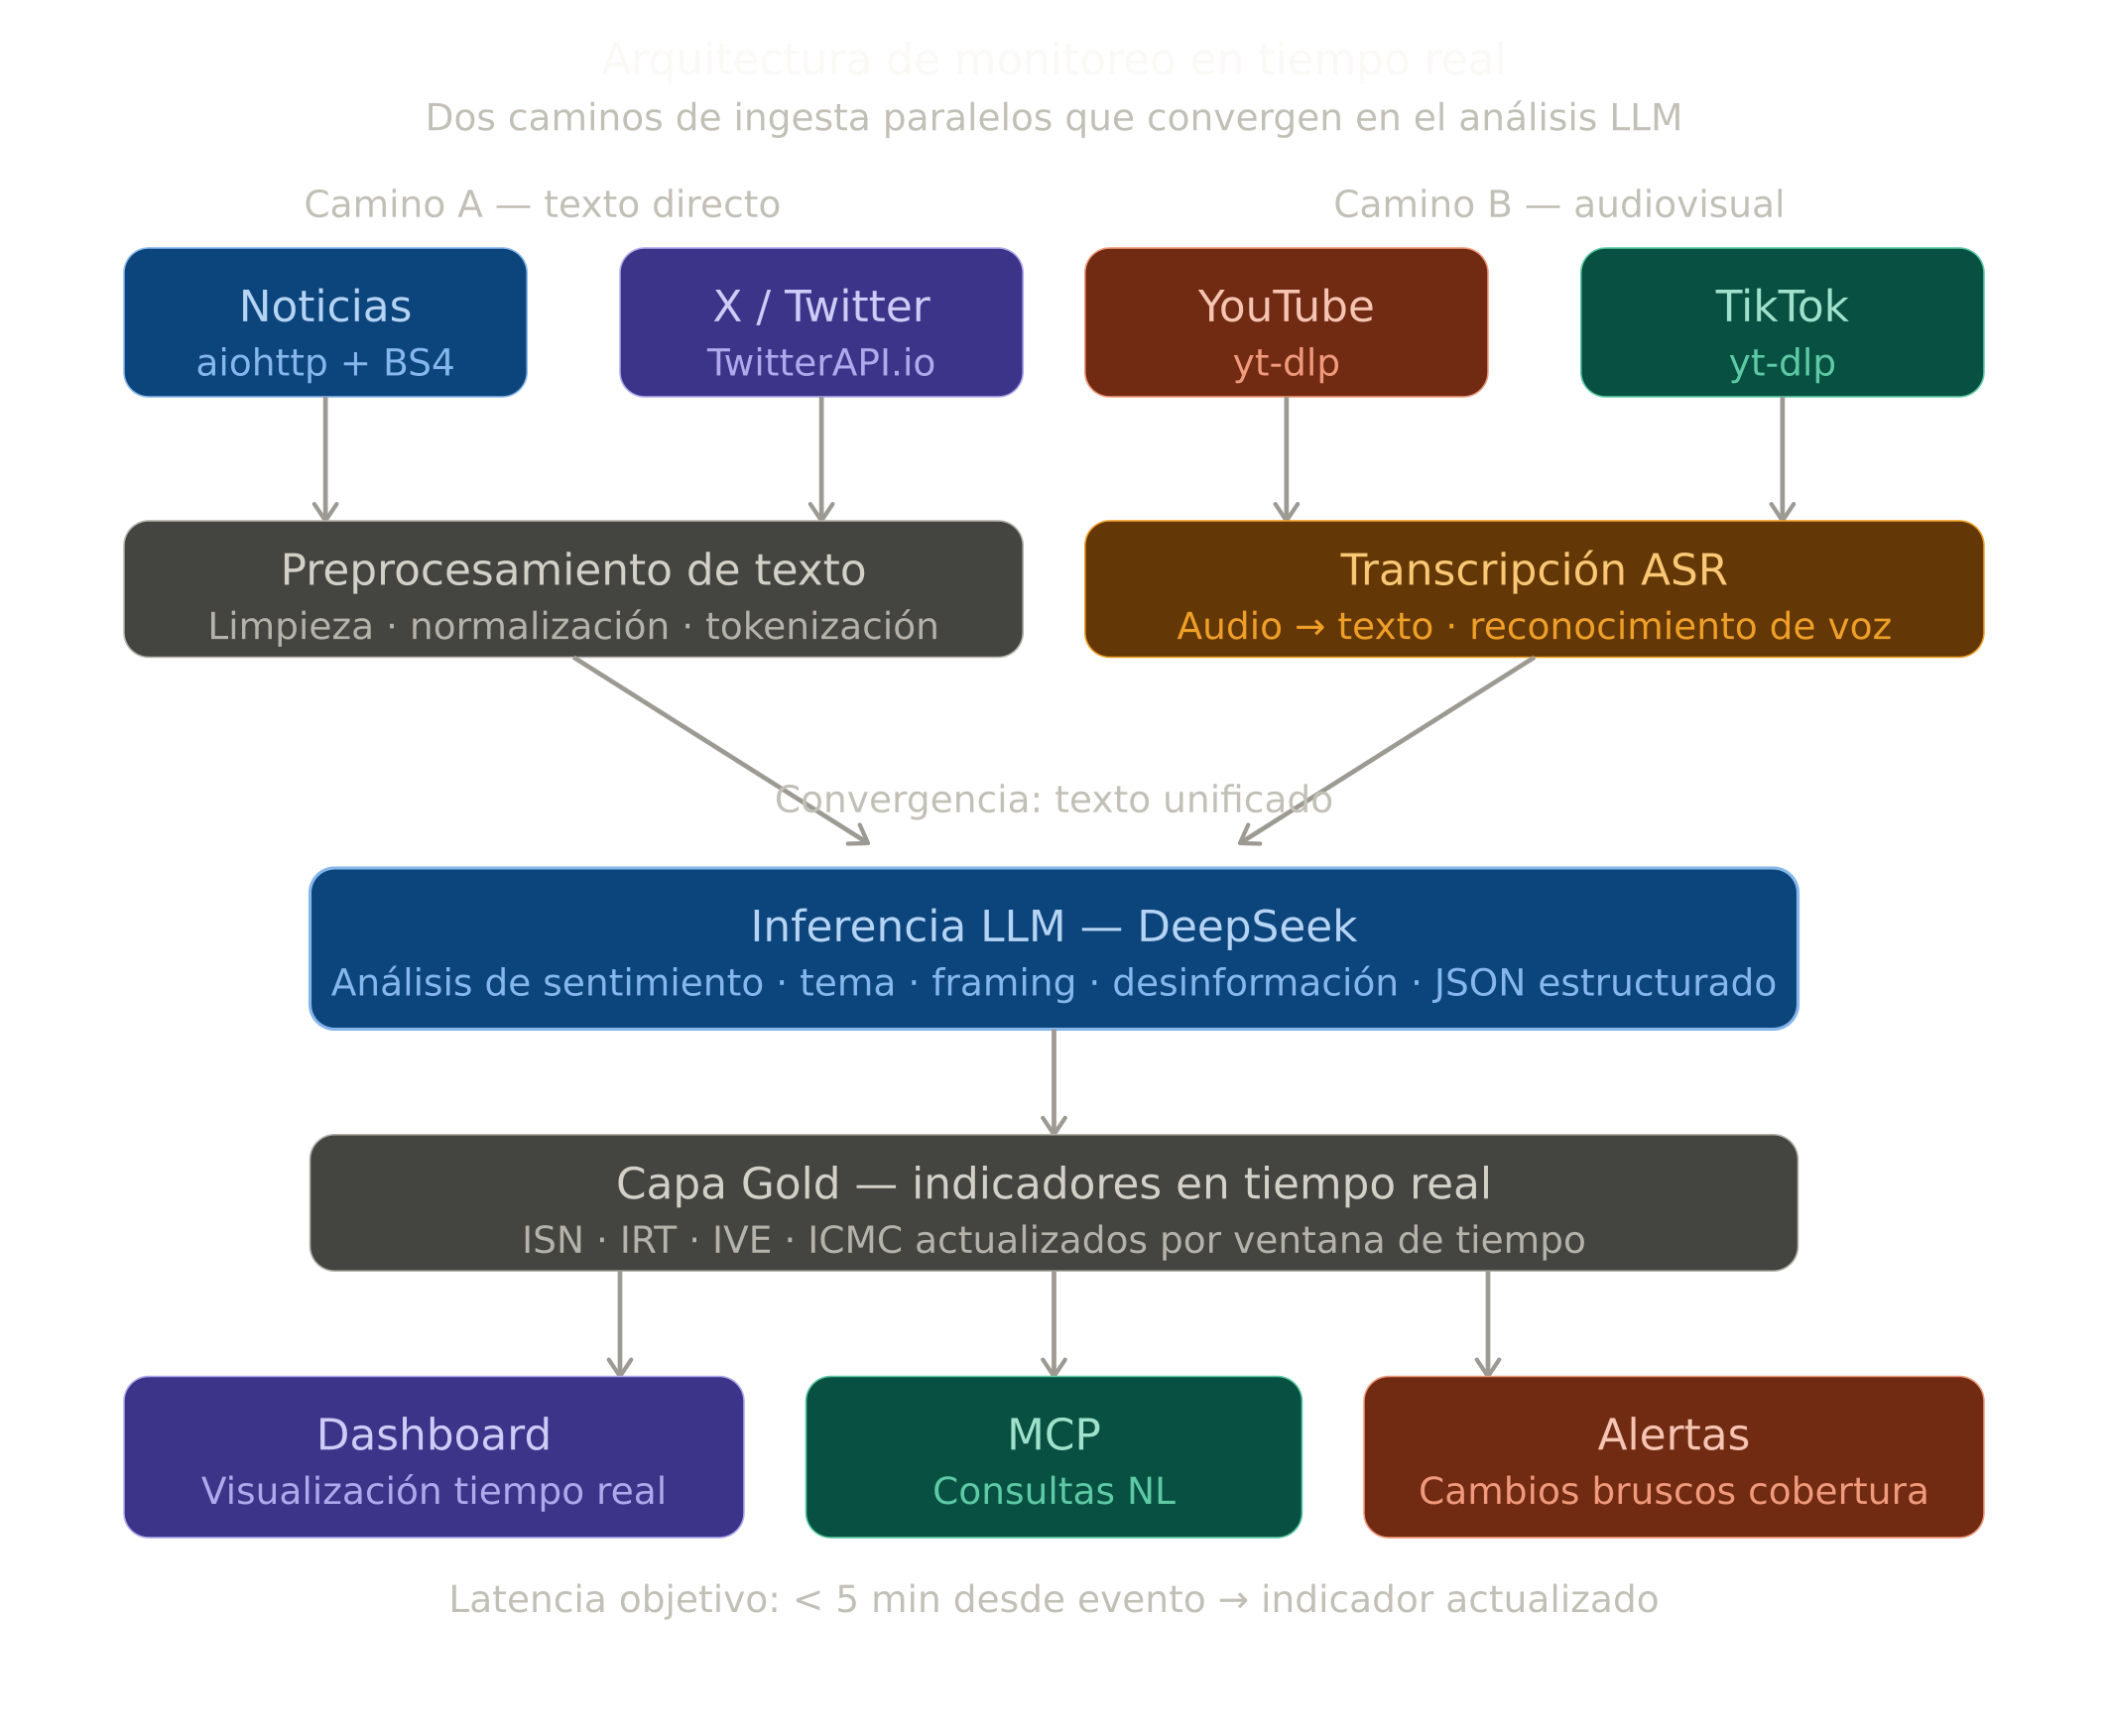
\includegraphics[width=0.90\textwidth]{2/figures/realtime_architecture.jpg}
        \caption[Arquitectura de procesamiento en tiempo real para monitoreo de percepción electoral]{Arquitectura de un sistema de monitoreo electoral en tiempo real: ingesta de datos en streaming, preprocesamiento, inferencia LLM paralela y actualización de dashboards de visualización.\\
            Fuente: Elaboración propia basada en \cite{mc_garcia2025real_time}.}
        \label{fig:realtime_architecture}
    \end{center}
\end{figure}
 
% ──────────────────────────────────────────────────────────────
\subsection{Indicadores de Percepción Electoral}
% ──────────────────────────────────────────────────────────────
 
Los \textbf{indicadores de percepción electoral} son métricas cuantitativas derivadas del análisis de datos del ecosistema digital que permiten operacionalizar y medir de manera sistemática la percepción pública hacia candidatos, partidos, temas y el proceso electoral en general \parencite{mc_ceron2017social}. En la presente investigación se definen los siguientes indicadores principales:
 
El \textbf{Índice de Sentimiento Neto} (ISN) mide la diferencia entre la proporción de publicaciones con sentimiento positivo y negativo hacia una entidad política en un período determinado, calculado mediante la Ecuación \ref{eq:isn}:
 
\begin{equation}\label{eq:isn}
\phantomsection
ISN_{(e,t)} = \frac{P_{pos}(e,t) - P_{neg}(e,t)}{P_{total}(e,t)} \times 100
\end{equation}
\myequations{Índice de Sentimiento Neto para entidades políticas}
 
Donde:
\begin{conditions}
P_{pos}(e,t)    & número de publicaciones con sentimiento positivo hacia la entidad $e$ en el período $t$ \\
P_{neg}(e,t)    & número de publicaciones con sentimiento negativo hacia la entidad $e$ en el período $t$ \\
P_{total}(e,t)  & número total de publicaciones que mencionan a la entidad $e$ en el período $t$
\end{conditions}
 
El \textbf{Índice de Relevancia Temática} (IRT) mide la importancia relativa de un tema en el corpus en un período dado, calculado como la proporción de publicaciones asignadas a ese tema sobre el total del corpus en ese período. El \textbf{Índice de Velocidad de Emergencia} (IVE) mide la rapidez con la que un tema nuevo gana relevancia, calculado como la derivada temporal del IRT. Estos tres indicadores, monitoreados conjuntamente en tiempo real, constituyen el núcleo analítico del sistema de inteligencia electoral propuesto.